\documentclass[11pt]{article}
\usepackage[letterpaper,margin=1in]{geometry}
\usepackage{listings}
\usepackage{url}
\usepackage{hyperref}
\usepackage{textcomp}
\usepackage{graphicx}
\usepackage{underscore}
\lstset{%
  basicstyle=\small\ttfamily,
  mathescape=true,
  upquote=true,
}

\usepackage{amsmath,amsbsy,amsfonts,amssymb,amsthm,color,dsfont,mleftright,commath}

\def\ddefloop#1{\ifx\ddefloop#1\else\ddef{#1}\expandafter\ddefloop\fi}

% \bbA, \bbB, ...
\def\ddef#1{\expandafter\def\csname bb#1\endcsname{\ensuremath{\mathbb{#1}}}}
\ddefloop ABCDEFGHIJKLMNOPQRSTUVWXYZ\ddefloop

% \cA, \cB, ...
\def\ddef#1{\expandafter\def\csname c#1\endcsname{\ensuremath{\mathcal{#1}}}}
\ddefloop ABCDEFGHIJKLMNOPQRSTUVWXYZ\ddefloop

% \vA, \vB, ..., \va, \vb, ...
\def\ddef#1{\expandafter\def\csname v#1\endcsname{\ensuremath{\boldsymbol{#1}}}}
\ddefloop ABCDEFGHIJKLMNOPQRSTUVWXYZabcdefghijklmnopqrstuvwxyz\ddefloop

% \valpha, \vbeta, ...,  \vGamma, \vDelta, ...,
\def\ddef#1{\expandafter\def\csname v#1\endcsname{\ensuremath{\boldsymbol{\csname #1\endcsname}}}}
\ddefloop {alpha}{beta}{gamma}{delta}{epsilon}{varepsilon}{zeta}{eta}{theta}{vartheta}{iota}{kappa}{lambda}{mu}{nu}{xi}{pi}{varpi}{rho}{varrho}{sigma}{varsigma}{tau}{upsilon}{phi}{varphi}{chi}{psi}{omega}{Gamma}{Delta}{Theta}{Lambda}{Xi}{Pi}{Sigma}{varSigma}{Upsilon}{Phi}{Psi}{Omega}{ell}\ddefloop

\newcommand\braces[1]{\{#1\}}

\theoremstyle{definition}
\newtheorem{problem}{Problem}
\newenvironment{solution}{\noindent\emph{Solution.}}{\hfill$\square$}

%-------------------------------------------------------------------------------

\title{COMS 4771 Spring 2017 Homework 4}
\author{Jin Tack Lim, jl4312
  }
\date{%
  }

\begin{document}
\maketitle


%-------------------------------------------------------------------------------

Problem 1.

(a) 

Consider the case in Figure~\ref{fig:one-rest}. There are three cases: C1, C2 and C3. Using
'one vs. rest', we can draw three lines, which classify a sample to either a
specific class or other classes. The whole space is divided into seven regions.
Out of seven, there are three regions that is classified to a specific class
clearly: R2 is C2, R4 is C3 and R6 is C1.  However there is a region that
doesn't fit into any class: R1. Also, there are regions that are classified
into multiple classes: R3, R5, R7.

So, this example showed that 'one vs. rest' has some drawbacks.

\begin{figure}[h]
  \centering
  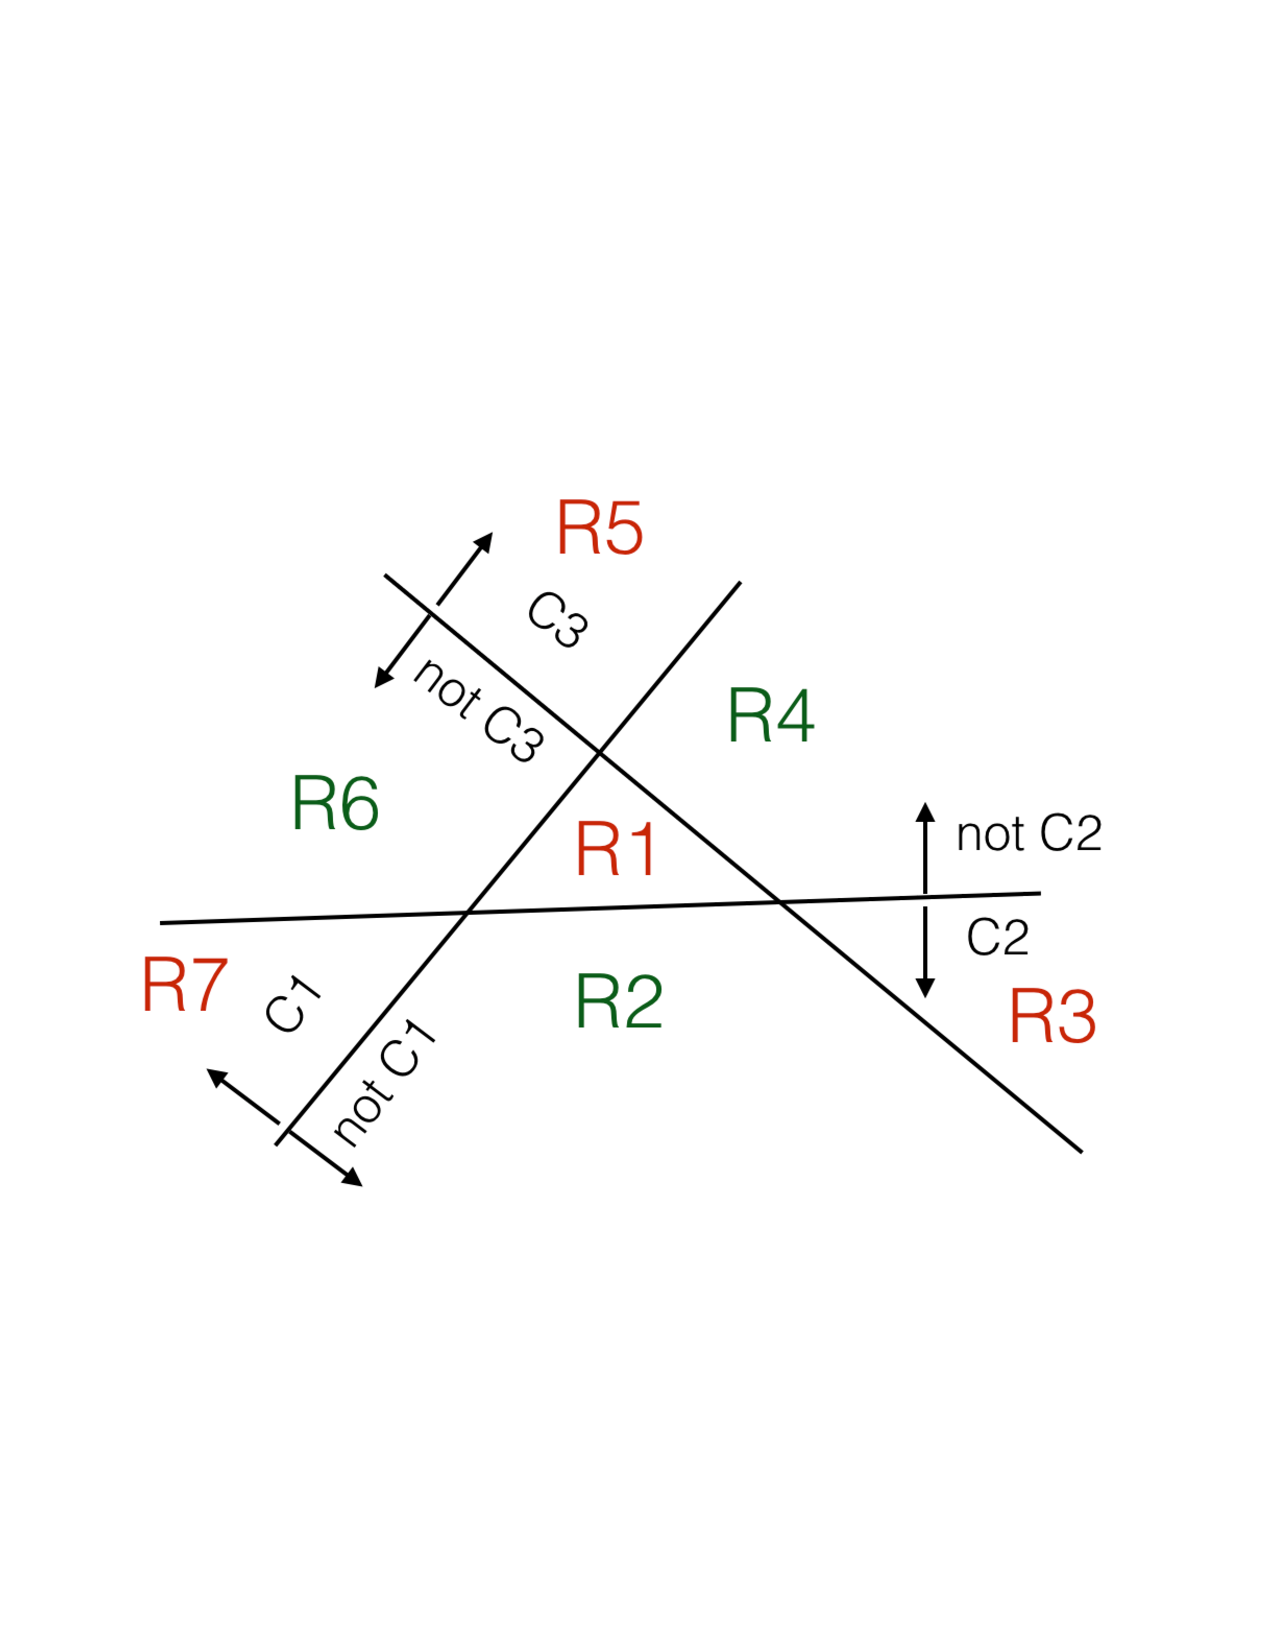
\includegraphics[width=\textwidth]{one-rest}
  \caption{One vs. rest}
  \label{fig:one-rest}
\end{figure}

(b)

Consider the case in Figure~\ref{fig:one-one}. There are three cases: C1, C2 and C3. Using
'one vs. one', we can draw three lines (3*2/2), which classify a sample to one
of two classes for each pair of classes.  The whole space is divided into seven
regions.  Out of seven, six regions are clearly classified into a specific
class: R6 and R7 are C1, R2 and R3 are C2, R4 and R5 are C3.  However R1 can't
be classified because there is no single winner: 1 vote for each classes.

So, this example showed that 'one vs. one' also has some drawbacks.

\begin{figure}[h]
  \centering
  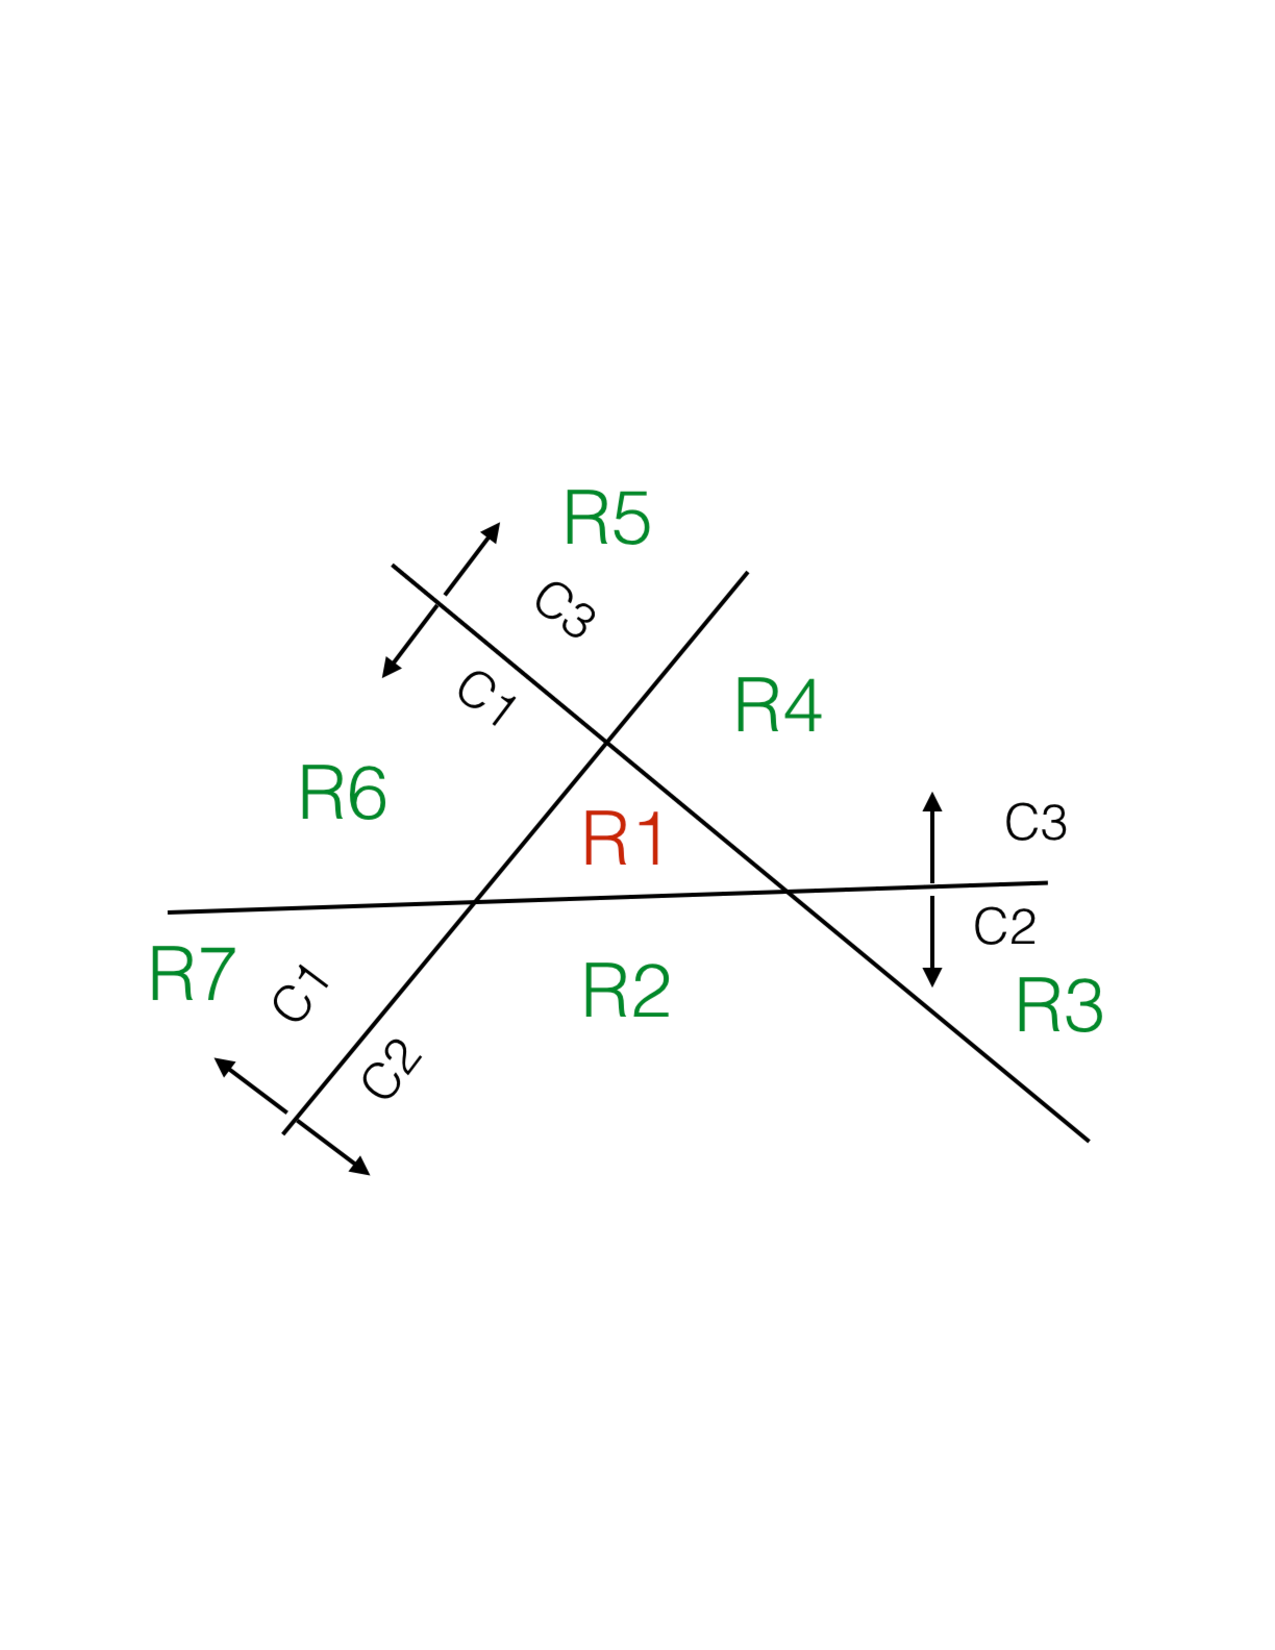
\includegraphics[width=\textwidth]{one-one}
  \caption{One vs. One}
  \label{fig:one-one}
\end{figure}

(c)

\end{document}

